%%==================================================
%% chapter01.tex for SJTU Master Thesis
%% based on CASthesis
%% modified by wei.jianwen@gmail.com
%% version: 0.3a
%% Encoding: UTF-8
%% last update: Dec 5th, 2010
%%==================================================

%\bibliographystyle{sjtu2} %[此处用于每章都生产参考文献]
\chapter{背景介绍}
\label{chap:background}

移动无线网络中的一个基本问题是如何在系统可靠性与网络传输性能之间进行有效平衡,对于高速移动网络而言,首先要保证其系统可靠性以实现信息的可靠传输;而无线局域网络则更关注网络的传输性能,包括网络吞吐量及覆盖范围等。其中信道状态和链路质量作为无线网络可靠性与传输性能的衡量指标,同时也是网络运行与优化的重要参数,因此两者的准确高效的测量对于移动网络中可靠性与传输性能的有效平衡至关重要。本文主要针对高速移动网络和无线局域网络中的信道估计与链路测试问题,对移动网络的通信质量测试进行详细分析,并通过算法设计、系统实现与实验测试对移动网络通信质量测试算法进行性能评估。

\section{移动无线网络}
\label{sec:mobile}


\subsection{高速移动网络}
\label{sec:gsmr}

在高速铁路的快速发展的过程中,列车的安全稳定运行至关重要,要实现高铁的安全稳定高速运行,必须实时地对整个高铁系统进行安全监测。其中列控系统保证高铁系统的可靠运行,GSM-R无线网络则是列控系统中的关键环节,同时又是系统中最脆弱的部分。GSM-R网络是专门应用于铁路环境中的综合数字调度移动通信网络,如图 \ref{fig:gsmrservice} 所示,GSM-R网络承载了高速铁路的列车运行状态数据传输、列车控制数据传输、区间移动公务通信、应急指挥通信等业务,因此对GSM-R网络进行实时监测具有重要意义。

\begin{figure}[!htp]
\centering
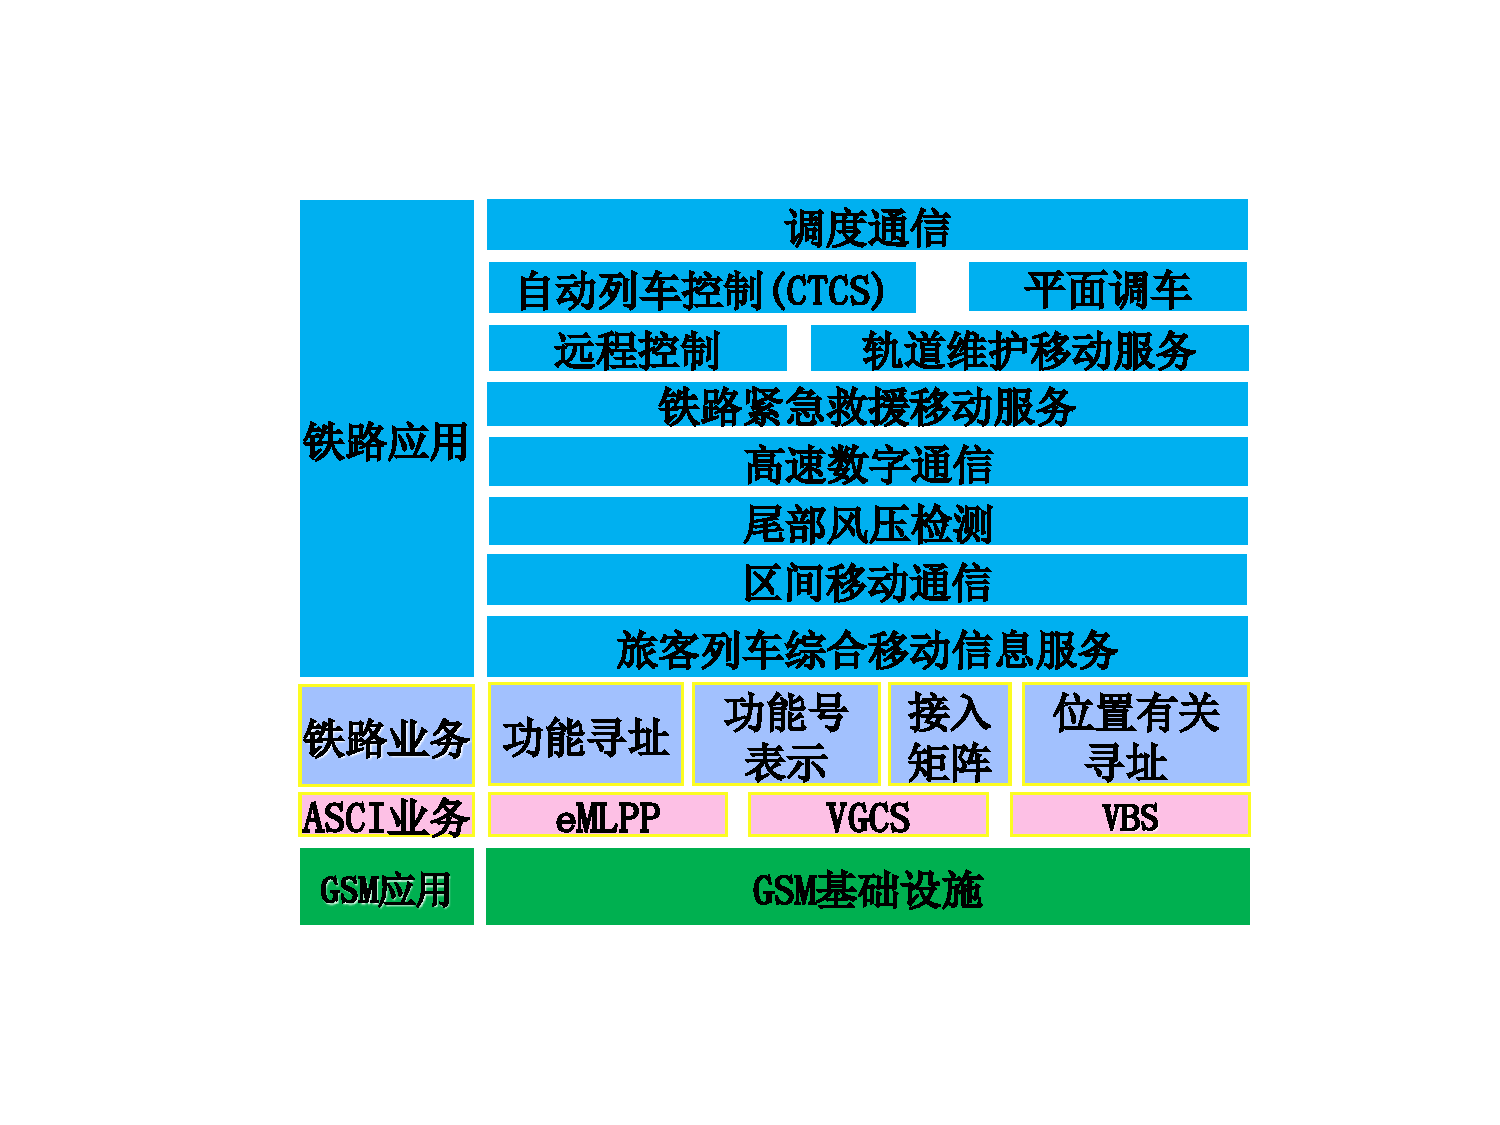
\includegraphics[width=0.6\textwidth]{chap1/gsmrservice.pdf}
\bicaption[fig:gsmrservice]{GSM-R网络业务模型}{GSM-R网络业务模型}{Fig}{Service model of GSM-R networks}
\end{figure}

目前我国的GSM-R数字移动通信系统由七个子系统构成:网络交换子系统(SSS)、基站子系统(BSS)、操作维护子系统(OSS)、通用分组无线业务子系统(GPRS)、智能网子系统(IN)、固定接入交换子系统(FAS)和终端子系统,如图 \ref{fig:gsmr} 所示。GSM-R系统的各个功能单元通过不同的接口进行连接,使各组成单元在物理上和逻辑上遵守特定的协议。GSM-R系统测试的主要应用到的接口有空中接口、Abis接口、A接口、PRI接口等,其中空中接口是移动台与基站之间的通信接口,用于移动台与GSM-R系统固定部分之间的通信,其物理连接通过无线链路实现,它的特点是完全标准化。

在GSM-R网络的通信过程中,大部分的信令都是和移动台相关,从图 \ref{fig:gsmr} 中可以看出,虽然移动台只和基站之间存在接口,但发往基站和从基站发往移动台的信令消息中还包括了移动台与GSM-R网络中其他设备之间的通信信息,即要在无线接口上传输各种不同的协议。同时,由于空中接口为无线链接,其可靠性是GSM-R网络能够正常运行的基础,因此需要对GSM-R的空中接口进行实时监测 \cite{baldini2010early}。

\begin{figure}[!htp]
\centering
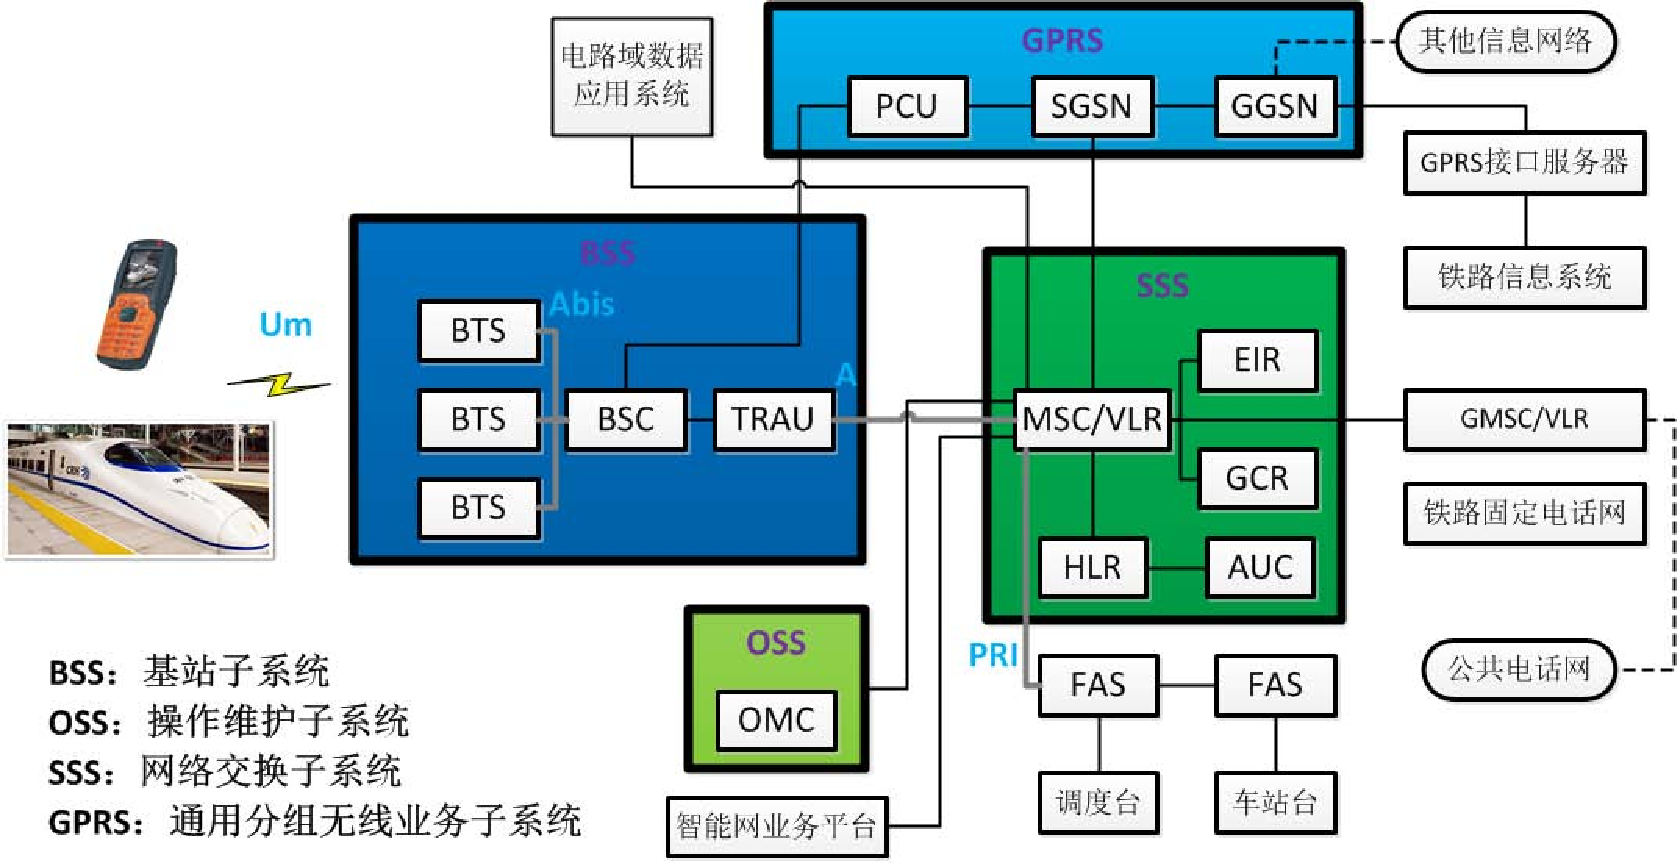
\includegraphics[width=0.9\textwidth]{chap1/gsmr.pdf}
\bicaption[fig:gsmr]{GSM-R网络基本结构}{GSM-R网络基本结构}{Fig}{Architecture of GSM-R networks}
\end{figure}

\subsection{无线局域网络}
\label{sec:80211n}

近年来,无线业务的流量和带宽需求不断提高,使得基于802.11n的无线局域网络(Wireless Local Area Networks, WLANs)经历了快速的发展,同时由于智能手机等移动终端的迅猛发展,802.11n网络将会得到进一步的发展 \cite{Bala2010wifi}。802.11n网络一方面能够有效提升网络性能,同时也使得链路质量的测试与建模更为复杂。

802.11n网络的显著特点是采用了MIMO-OFDM及其相关技术,从而有效地提升网络的传输性能。在物理层方面,多天线技术有效提升网络吞吐量及覆盖范围,同时提高系统的稳定性,以及信道绑定技术等,更好地解决载波侦听、隐藏/暴露终端等问题;在链路层方面,802.11n网络采用帧聚合技术即多个帧共用一个MAC头部,同时降低ACK发送频率及发送/接收开销,提高传输效率,同时采用400ns的短保护间隔,以降低时间开销,并提高链路层吞吐量。

\begin{table}[!htp]
\renewcommand{\arraystretch}{1}
\bicaption[tab:feature]{802.11网络基本参数}{802.11网络基本参数}{Table}{Features and settings of 802.11 networks}
\centering
\begin{threeparttable}[b]
\begin{tabular}{ccccc}
\hline
         & 802.11a  & 802.11b    & 802.11g       & 802.11n \\
\hline
调制方式 & OFDM     & DSSS/CCK   & OFDM DSSS/CCK & SDM/OFDM \\
%\cline{2}
频率     & 5GHz     & 2.4GHz     & 2.4GHz        & 2.4/5GHz \\
%\cline{2}
信道带宽 & 20MHz    & 25MHz      & 25MHz         & 20/40MHz \\
%\cline{2}
传输速率 & 6-54Mbps & 5.5/11Mbps & 1-54Mbps     & 6-600Mbps \\
\hline
\end{tabular}
\end{threeparttable}
\end{table}

首先802.11n网络显著提升了无线局域网络的传输性能、覆盖范围及其兼容性。在传输速率方面,802.11n可以将无线局域网的传输速率由目前802.11a及802.11g提供的54Mbps,提高到300Mbps甚至高达600Mbps。得益于将多天线(Multiple Input Multiple Output, MIMO)与正交频分复用(Orthogonal Frequency Division Multiplexing, OFDM)技术相结合而应用的MIMO-OFDM技术,提高了无线传输质量,也使传输速率得到极大提升,如表 \ref{tab:feature} 所示;在覆盖范围方面,802.11n采用智能天线技术,通过多组独立天线组成的天线阵列,可以动态调整波束,保证让用户接收到稳定的信号,并可以减少其它信号的干扰。因此其覆盖范围可以扩大到好几平方公里,同时使无线局域网的移动性得到极大提高;在兼容性方面,802.11n采用了一种软件无线电技术,它是一个完全可编程的硬件平台,使得不同系统的基站和终端都可以通过这一平台的不同软件实现互通和兼容,这使得WLAN的兼容性得到极大改善。这意味着WLAN将不但能实现802.11n向前后兼容,而且可以实现WLAN与无线广域网络的结合,比如3G 网络。

\begin{table}[!htp]
\renewcommand{\arraystretch}{1}
\bicaption[tab:mcs]{802.11n网络MCS索引}{802.11n网络MCS索引}{Table}{MCS index of 802.11n}
\centering
\begin{threeparttable}[b]
\begin{tabular}{cccccc}
\hline
  \multirow{2}{*}{MCS} & \multirow{2}{*}{Modulation} & \multirow{2}{*}{Code Rate} & \multirow{2}{*}{Rate (Mbps)} & \multicolumn{2}{c}{Sensitivity (dBm)} \\
\cline{5-6}
  & & & & Typical & Max \\
\hline
  0 & BPSK & 1/2 & 6.5 & -94 & -85 \\
%\cline{2}
  1 & QPSK & 1/2 & 13.0 & -92 & -82 \\
%\cline{2}
  2 & QPSK & 3/4 & 19.5 & -90 & -80 \\
%\cline{2}
  3 & 16 QAM & 1/2 & 26.0 & -87 & -77 \\
%\cline{2}
  4 & 16 QAM & 3/4 & 39.0 & -84 & -73 \\
%\cline{2}
  5 & 64 QAM & 2/3 & 52.0 & -79 & -69 \\
%\cline{2}
  6 & 64 QAM & 3/4 & 58.5 & -78 & -68 \\
%\cline{2}
  7 & 64 QAM & 5/6 & 65.0 & -76 & -67 \\
\hline
\end{tabular}
\end{threeparttable}
\end{table}

另一方面,802.11n网络链路质量的测试与建模更为复杂,如表 \ref{tab:mcs} 所示。第一,802.11n网络的多种配置提高了链路质量测试的复杂度,需要对所有可能的物理层与链路层配置进行采样测试,同时使得链路质量的建模变得复杂;第二,802.11n网络的链路质量与信道状态(Packet Delivery Ratio - Received Signal Strength, PDR-RSS)模型呈现过渡窗口,而并非传统无线网络中的近似线性关系;第三,移动网络的信道状态与链路质量更容易受到无线传播环境及通信终端的移动性的影响,从而影响到链路质量测试与建模的精度。
%
%\begin{figure}[!htp]
%\centering
%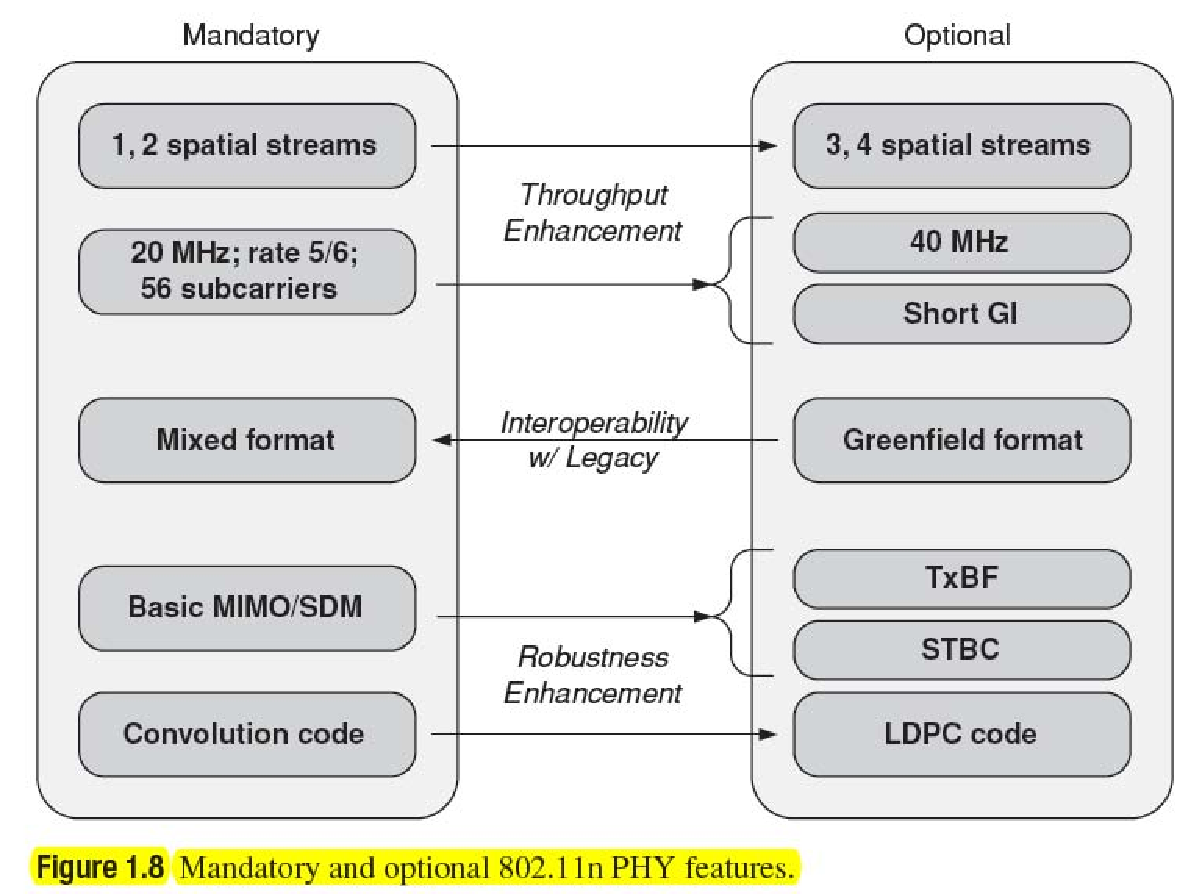
\includegraphics[width=0.5\textwidth]{chap1/PHYfeather.pdf}
%\bicaption[fig:phyfeather]{802.11n网络PHY特性}{802.11n网络PHY特性}{Fig}{Feather of 802.11n Networks}
%\end{figure}
%
%\subsubsection{物理层}
%\begin{itemize}
%  \item Spatial Diversity
%  \item Channel Bonding
%\end{itemize}
%
%
%\begin{figure}[!htp]
%\centering
%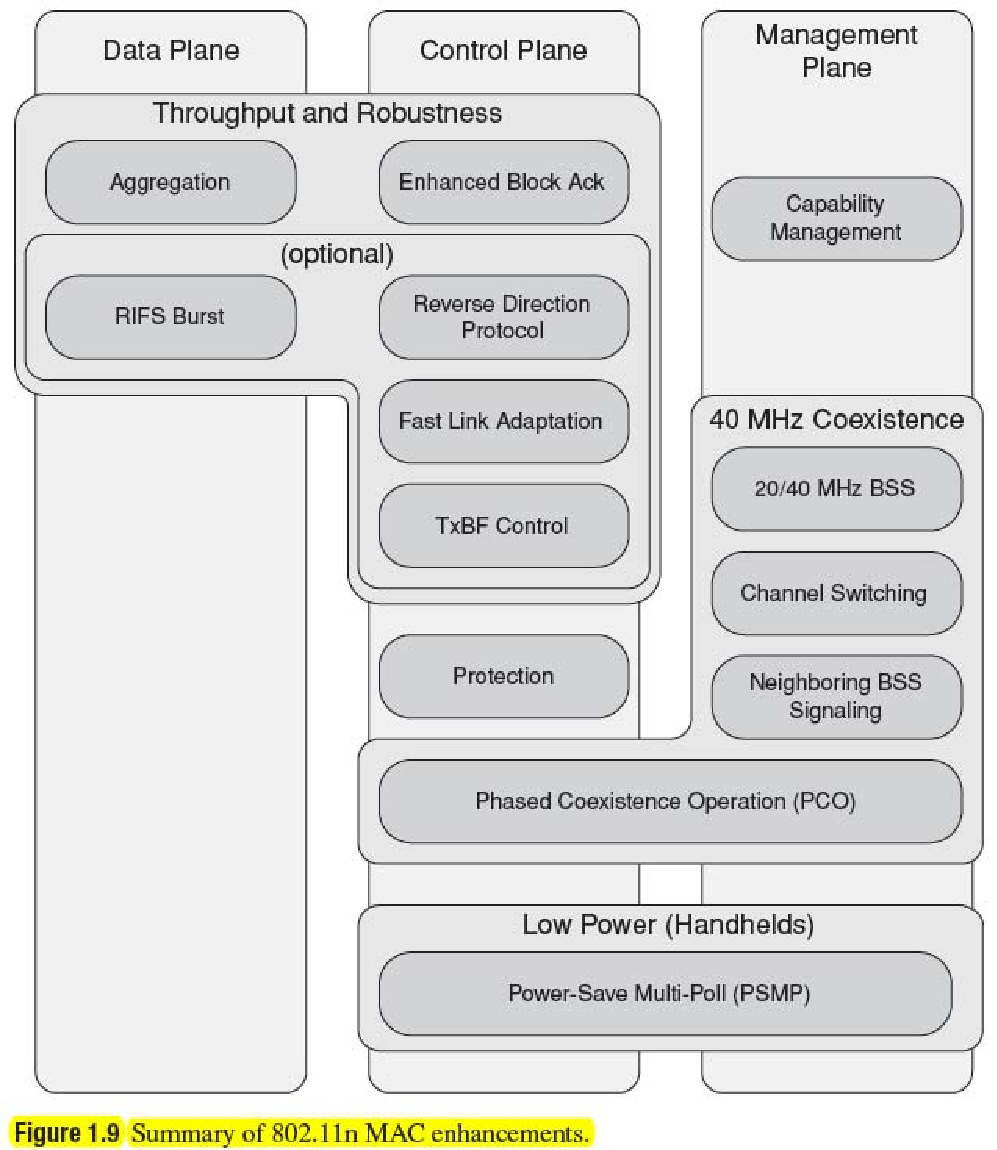
\includegraphics[width=0.5\textwidth]{chap1/MACfeather.pdf}
%\bicaption[fig:macfeather]{802.11n网络MAC特性}{802.11n网络MAC特性}{Fig}{Feather of 802.11n Networks}
%\end{figure}
%
%\subsubsection{链路层}
%\begin{itemize}
%  \item Frame Aggregation
%  \item Streamlined ACK
%\end{itemize}

%\begin{table}[!htp]
%\renewcommand{\arraystretch}{1}
%\bicaption[tab:mcs]{802.11n网络MCS索引}{802.11n网络MCS索引}{Table}{MCS index of 802.11n}
%\centering
%\begin{threeparttable}[b]
%\begin{tabular}{c|c|c|ccc}
%\hline
%  Channel & MCS & Rate(Mbps) & $\beta_-$ & $\beta_0$ & $\beta_+$ \\
%\hline
%  \multirow{8}{*}{HT20/LGI} & 0 &  6.5 & -70 & -65 & -60 \\
%\cline{2}
%                            & 1 & 13.0 & -70 & -65 & -60 \\
%\cline{2}
%                            & 2 & 13.0 & -70 & -65 & -60 \\
%\cline{2}
%                            & 3 & 13.0 & -70 & -65 & -60 \\
%\cline{2}
%                            & 4 & 13.0 & -70 & -65 & -60 \\
%\cline{2}
%                            & 5 & 13.0 & -70 & -65 & -60 \\
%\cline{2}
%                            & 6 & 13.0 & -70 & -65 & -60 \\
%\cline{2}
%                            & 7 & 13.0 & -70 & -65 & -60 \\
%\hline
%  \multirow{8}{*}{HT20/SGI} & 0 &  6.5 & -70 & -65 & -60 \\
%\cline{2}
%                            & 1 & 13.0 & -70 & -65 & -60 \\
%\cline{2}
%                            & 2 & 13.0 & -70 & -65 & -60 \\
%\cline{2}
%                            & 3 & 13.0 & -70 & -65 & -60 \\
%\cline{2}
%                            & 4 & 13.0 & -70 & -65 & -60 \\
%\cline{2}
%                            & 5 & 13.0 & -70 & -65 & -60 \\
%\cline{2}
%                            & 6 & 13.0 & -70 & -65 & -60 \\
%\cline{2}
%                            & 7 & 13.0 & -70 & -65 & -60 \\
%\hline
%\end{tabular}
%\end{threeparttable}
%\end{table}


\section{通信质量测试}
\label{sec:measure}

对于高速移动网络GSM-R与无线局域网络802.11n通信质量测试而言,其目标都是实现系统可靠性与网络传输性能的有效平衡,但是两者的侧重点不同,前者主要保证网络的可靠运行,而后者主要实现传输性能的提升。无线网络通信质量通常由信道状态与链路质量进行衡量,而信道状态是链路质量的基础,因此对于GSM-R网络而言,其关键是如何在高速移动情况下实现信道状态的可靠估计,同时在保证测试精度的前提下尽量降低测试开销,进而完成上层的链路质量测试以保证系统可靠性;而对于移动802.11n网络,由于其移动性与多配置的特性,主要难点是如何实现实时的链路质量测试与建模,从而实现不同网络状态下网络的有效配置,以提高网络传输性能。

\subsection{物理层信道状态估计}
\label{sec:phy}

无线传播测量与信道状态估计在移动网络中发挥重要作用,并广泛应用于其他上层应用中,例如无线覆盖评估、信道接入、功率控制及小区切换等 \cite{Austin1994}\cite{itoh2002performance}\cite{zhang1996analysis}\cite{zhu2005performance}。文献 \cite{andersen1995propagation} \cite{sarkar2003survey} 给出了无线网络中无线传播模型及其测试方法,文献 \cite{Ostlin2008itu} 以国际电信联盟(International Telecommunication Union, ITU)相关规定为基础提出点到面无线传输服务的无线预测模型,\cite{Akhoondzadeh2007modifi} 和 \cite{medeisis2000use} 分别基于最小均方差和Levenberg-Marquardet方法提出改进Okumura-Hata传播模型。以上的无线传播模型与测试方法主要集中于路径损耗与阴影衰落,当考虑到移动无线网络中的多径衰落时,主要问题是如何对接收信号强度进行估计,以准确反映网络当前的链路质量。

针对这一问题,William C. Y. Lee在1985年提出移动网络信号强度采样算法 \cite{lee1985estimate},该算法分析了瑞利衰落情况下接受信号强度本地均值的估计问题,并给出合适的统计区间与采样点数的参数设置。Mark D. Austin在其蜂窝网络的切换算法中对莱斯衰落条件下的采样算法进行了推导 \cite{Austin1994},得到统计区间与采样点数的近似解,但是该算法过程复杂且计算量较大。David de la Vega在2009年提出通用Lee氏采样算法 \cite{Vega2009},在不需要知道多径衰落具体分布的条件下,利用实测采样信号进行估计,得到实际网络环境所需要的统计区间与采样点数。由于高速铁路无线环境的复杂性及其对安全性的特殊要求,以上的本地均值估计算法难以在较低的测试开销条件下实现可靠的测试精度,不符合高铁环境实时测试的要求,因此无法直接应用于GSM-R网络中。

由于高速铁路沿线地形复杂多变,一条线路通常会经过山地、平原、隧道和高架等地形,从而造成GSM-R网络无线传播环境的复杂性。同时高速铁路无线传播环境大多较为平坦,同时为了尽量保证GSM-R网络的可靠性,基站位置通常距离高铁线路很近,而且小区半径一般设置为3-6km,从而造成移动终端与基站之间一般存在直射路径(Line of Sight, LOS),因此GSM-R网络的无线传播应该刻画为莱斯衰落。对于莱斯衰落信道的参数估计已有大量相关工作,包括基于学习训练机制 \cite{bjornson2010framework}、最大似然估计(Maximum Likelihood, ML) \cite{sijbers1998maximum} 以及期望最大化算法(Expectation Maximization, EM)\cite{marzetta1995algorithm}。因此GSM-R网络的信道状态估计问题实为莱斯衰落信道下本地均值估计,如何通过莱斯衰落参数估计,确定信道状态测试的采样参数。

\subsection{链路层链路质量测试}
\label{sec:mac}

无线网络中基于实测数据的PDR-RSS模型存在大量研究,多数早期的工作主要针对静态无线网络中的离线PDR-RSS模型 \cite{kolar2011mesh} \cite{reis2006model},同时实测PDR-RSS模型广泛应用于其他上层应用中,包括容量分析 \cite{kashyap2007capacity} 和速率控制 \cite{chen2011ram} \cite{judd2008efficient} 等。文献 \cite{10.1109/TMC.2009.87} 通过实验与仿真的结合,提出移动无线网络的可重复测量方法,文献 \cite{kim2010sybot} 同样提出针对移动网络的频谱测量方法,但是只对RSS进行测量而忽略链路质量。以上的移动无线网络测量方法都基于传统802.11a/b/g网络,而无法直接应用于802.11n网络中。由于802.11n网络采用MIMO-OFDM技术,导致PDR-RSS模型存在过渡窗口,从而增加了链路质量测试与建模的复杂度。近期许多工作针对802.11n 网络的实验特性进行了详细分析 \cite{Halperin2010predictable} \cite{k.rayanchu:fluid:},其中文献 \cite{Halperin2010predictable} 利用802.11n 网络的MIMO-OFDM 特性提出基于信道状态信息(Channel State Information, CSI)的链路质量预测模型;文献 \cite{k.rayanchu:fluid:} 针对信道绑定技术,分析了信道带宽对无线局域网络性能的影响。以上针对802.11n网络的工作并未针对移动性进行分析,同时主要针对物理层而忽略链路层的影响。

信道状态与链路质量及其模型广泛应用于速率控制算法中 \cite{kim2009experimental} \cite{Pefkianakis:2010} \cite{zhang2008practical} \cite{Li:2012:ERA:2348543.2348585},许多算法应用于Linux平台无线驱动中,例如采用Minstrel算法 \cite{minstrel} 的\textit{mac80211} 及Atheros \cite{wong2008wireless}的\textit{ath9k} 无线驱动,但是以上的算法都采用固定指数加权平均(Exponential Weighted Moving Average, EWMA)进行链路质量测试,仅适用于静态802.11网络。针对移动无线网络的速率控制算法主要针对RSS测量 \cite{chen2011ram} \cite{judd2008efficient},并利用静态PDR-RSS模型进行链路质量预测,但是其预测精度容易受802.11n网络的MIMO-OFDM配置的影响。许多上层应用考虑到在线PDR测试算法,比如入侵信号检测 \cite{5620919} 与拥塞控制 \cite{floyd2000equation} 等,但是并不考虑链路质量建模与速率控制问题。以上速率控制算法主要利用静态PDR-RSS模型 \cite{kashyap2007capacity} \cite{kolar2011mesh} \cite{reis2006model},同时只利用单一指标,即链路层PDR或物理层RSS,进行链路质量预测与速率控制 \cite{judd2008efficient} \cite{zhang2008practical}。

\section{本章小结}

本章主要介绍了移动网络通信质量测试,针对移动网络中可靠性与传输性能的有效平衡,提出信道状态与链路质量测试问题。首先对于高速移动网络GSM-R而言,首要问题是保证系统的可靠性,因此需要对无线接口进行实时监测,但由于移动终端的高速移动性及传播环境的复杂性,对信道状态估计的精度与开销带来极大挑战。其次在无线局域网络中,MIMO-OFDM技术能够有效地提升网络的传输性能,但同时其多配置的特性给链路质量测试与建模带来新的问题,而通信终端的移动性又进一步降低了链路质量测试的精度。因此本文针对移动网络中信道状态及链路质量测试问题,提出动态测试算法以根据当前网络状态调整测试参数,从而保证网络的可靠运行及传输性能。本文的章节安排如下,第二章主要介绍信道状态采样与估计,针对GSM-R网络的高速移动性与传播环境复杂性,提出接收信号强度动态测试算法,在保证一定测试精度的条件下降低测试开销,并通过系统设计与实现对该算法进行评估。第三章介绍链路质量测试与建模,主要解决移动802.11n网络中MIMO-OFDM配置及移动性对链路质量测试与建模带来的问题,提出在线测试与建模框架,在保证系统可靠性的前提下尽量提高系统吞吐量,最后通过系统实现与实验测试对其测试及传输性能进行评估。
